\documentclass[11pt]{article}
\usepackage[round]{natbib}
\usepackage{graphicx}
\usepackage{listings}
\usepackage{caption}
\usepackage{subcaption}
\usepackage{pgf}
\usepackage[most]{tcolorbox}
\usepackage[margin=1in]{geometry}
\usepackage{xcolor}
\usepackage{inconsolata}
\usepackage{cleveref}
\usepackage[inline]{enumitem}
\usepackage{dcolumn}
\usepackage{booktabs}

\usepackage[scaled]{helvet}
\renewcommand\familydefault{\sfdefault}
\usepackage[T1]{fontenc}

\definecolor{lightgray}{rgb}{.9,.9,.9}
\definecolor{darkgray}{rgb}{.4,.4,.4}
\definecolor{purple}{rgb}{0.65, 0.12, 0.82}
\definecolor{atomred}{RGB}{224, 108, 117}
\definecolor{atomwhite}{RGB}{250, 250, 250}

\lstdefinelanguage{JavaScript}{
  keywords={typeof, new, true, false, catch, function, return, null, catch, switch, var, if, in, while, do, else, case, break},
  keywordstyle=\color{blue}\bfseries,
  ndkeywords={class, export, boolean, throw, implements, import, this},
  ndkeywordstyle=\color{darkgray}\bfseries,
  identifierstyle=\color{black},
  sensitive=false,
  comment=[l]{//},
  morecomment=[s]{/*}{*/},
  commentstyle=\color{purple}\ttfamily,
  stringstyle=\color{atomred}\ttfamily,
  morestring=[b]',
  morestring=[b]"
}

\lstset{
   language=JavaScript,
   backgroundcolor=\color{atomwhite},
   extendedchars=true,
   basicstyle=\ttfamily\footnotesize,
   showstringspaces=false,
   showspaces=false,
   numbers=left,
   numberstyle=\ttfamily\footnotesize,
   numbersep=5pt,
   tabsize=2,
   breaklines=true,
   showtabs=false,
   captionpos=b,
   frame=single
}

\begin{document}

\title{On the Performance of String Search Algorithms for Deep Packet Inspection - Followup}
\author{Kieran Hunt}
\date{\today}
\maketitle

%TODO: Abstract

\section{Datasets}

\begin{table}[!htb]
\centering
\begin{tabular}{@{}lp{0.5\textwidth}ll@{}}
\toprule
Name & Description & $\mu$ Input Length & \#Inputs \\ \midrule
\textit{Dataset A} & Real-world DNS traffic & 109.61 & 10000 \\
\textit{Dataset B} & Full text of Alice in Wonderland by Lewis Carroll & 163780 & 1 \\
\textit{Dataset C} & Randomly generated DNS traffic with a payload size between 0 and 1500 bytes & 770.89 & 10000 \\
\textit{Dataset D} & Dataset C edited so that the payload just contains matches to the required rules & 770.89 & 10000 \\
\textit{Dataset E} & Dataset C edited so that each packet is filled with a random number of matches & 769.92 & 10000 \\
\textit{Dataset F} & Packets of fixed length completely filled with matches to the rules & 1500 & 10000
\end{tabular}
\caption{All datasets used in the tests}
\label{table-datasets}
\end{table}

\section{Processing Speed vs Input Length} \label{sec-processingspeecvsinputlength}

In a previous paper by \citet{hunt2016}, a selection of DNS traffic was used as input for the comparison between algorithm processing time and input length. The average length of a packet from that dataset was near 110 bytes. While that length made sense for dns traffic - notoriously low bandwidth usage - it did mean that a true reflection of algorithmic performance could not be obtained for longer length packets. A dataset of randomly generated DNS traffic was produced with a maximum length of 1500 bytes (the maximum transmission unit for ethernet) and a mean length of 770 bytes. The new set of packets is hereafter referred to as \textit{Dataset C}. More information can be found in Table \ref{table-datasetcinputlengthsummary}.

\begin{table}[!htb]
\centering
\begin{tabular}{@{}llllll@{}}
\toprule
Min & First Quartile & Median & Mean & Third Quartile & Max \\ \midrule
44 & 407 & 763.5 & 770.9 & 1136 & 1500 \\ \bottomrule
\end{tabular}
\caption{A summary of the input lengths in \textit{Dataset C}}
\label{table-datasetcinputlengthsummary}
\end{table}

Each of the four algorithms was tested for the same rules as in \citet{hunt2016} and with \textit{Dataset C} as input. Figure \ref{figure-individualalgorithmsvslength} shows a comparison between each of the algorithms.


\begin{figure}[!htb]
  \centering
  \begin{subfigure}[b]{0.48\textwidth}
      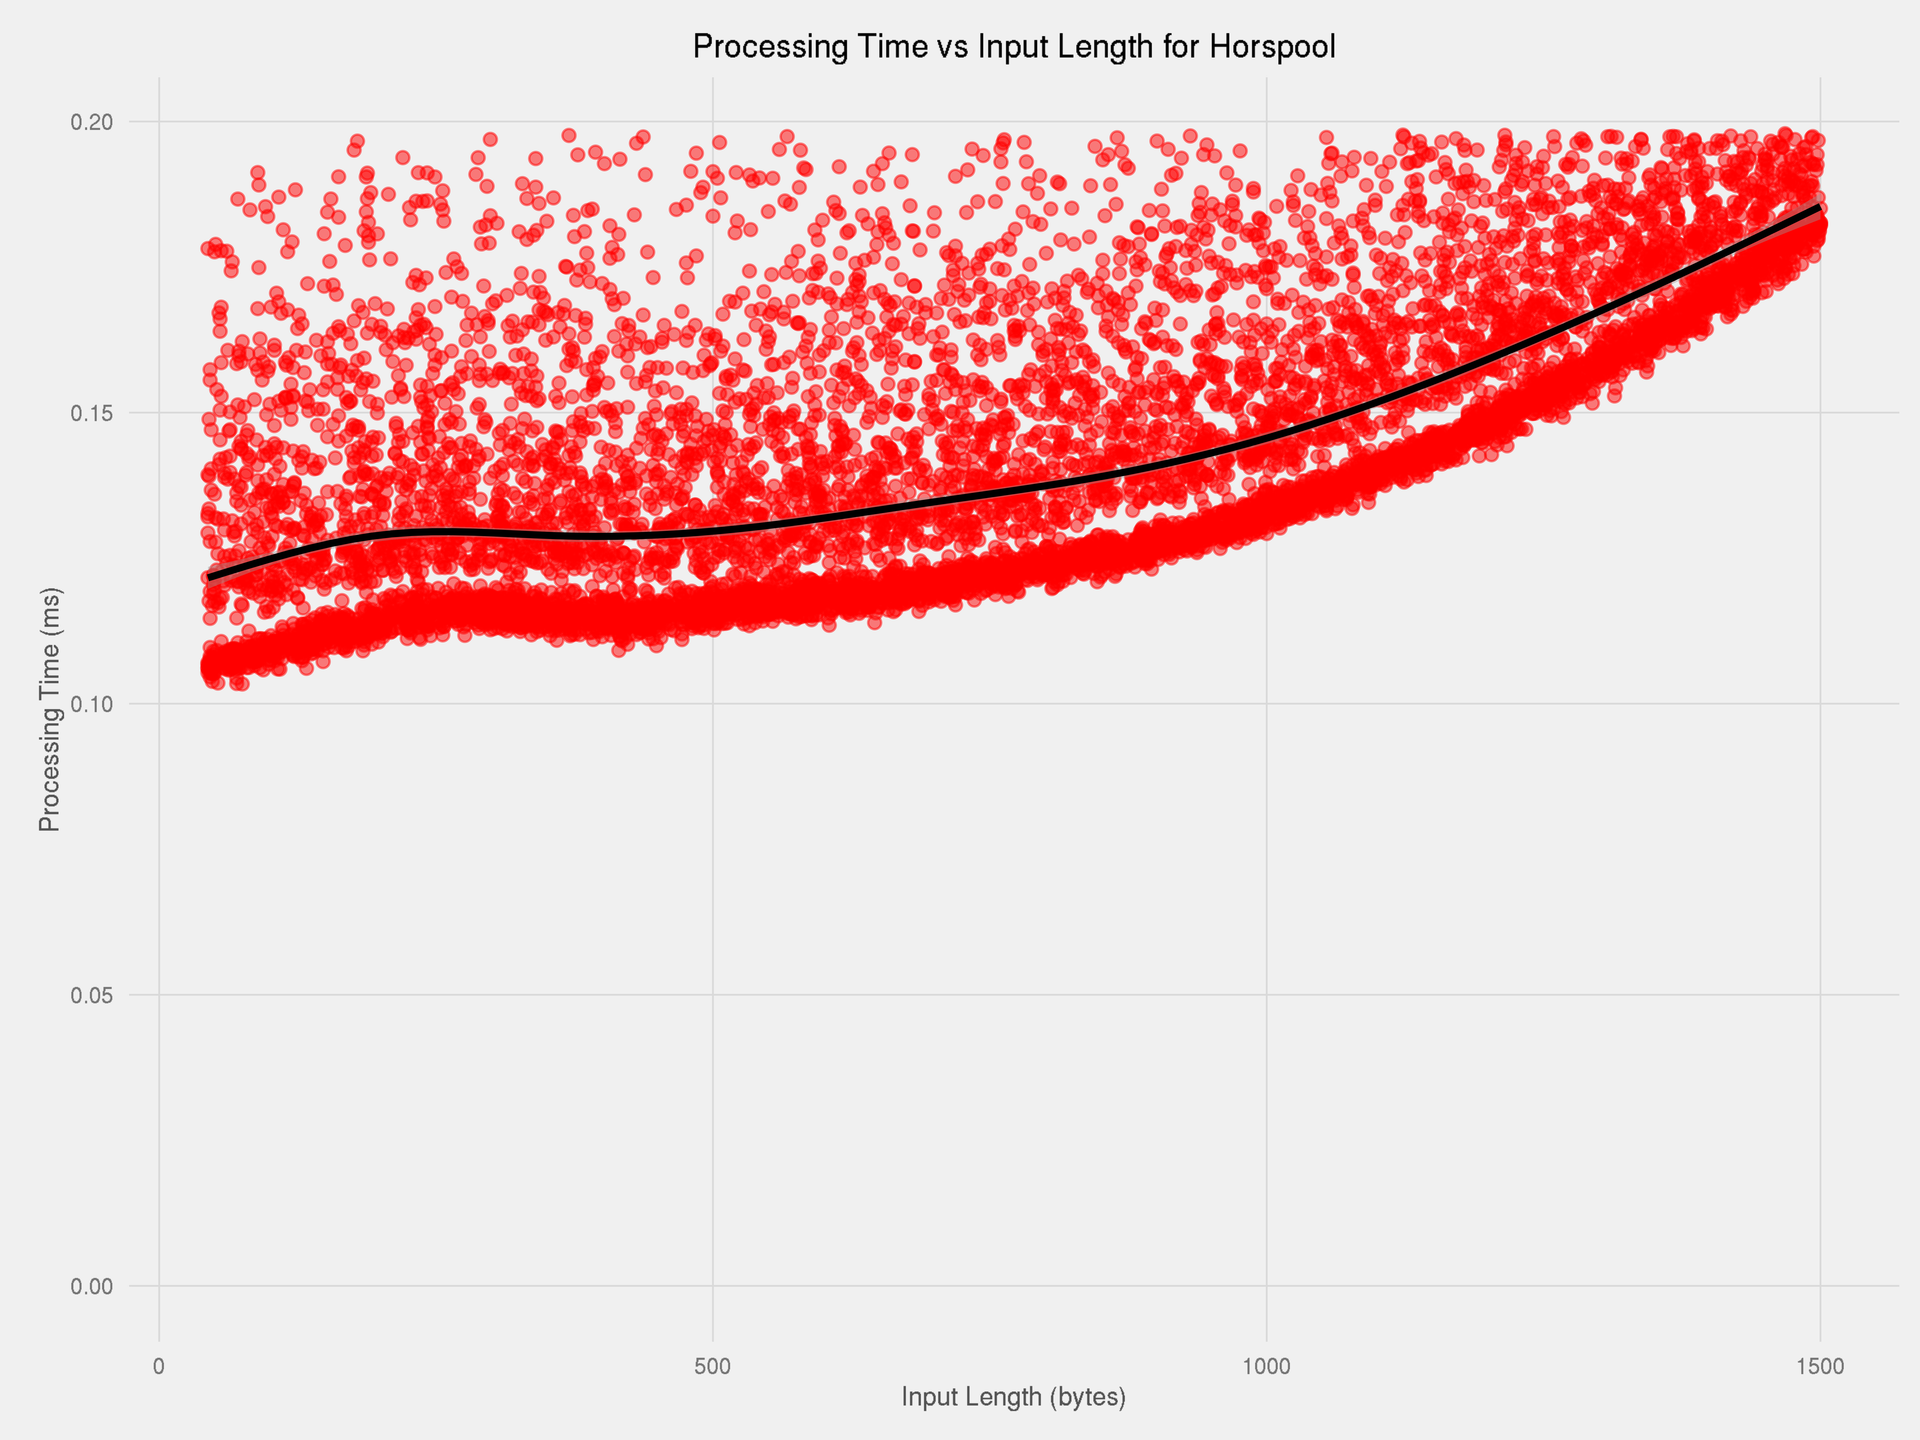
\includegraphics[width=\textwidth]{images/processing_speed_vs_input_length_no_matches_Horspool}
      \caption{Horspool}
      \label{figure-processingtimevslengthhorspool}
  \end{subfigure}
  \begin{subfigure}[b]{0.48\textwidth}
      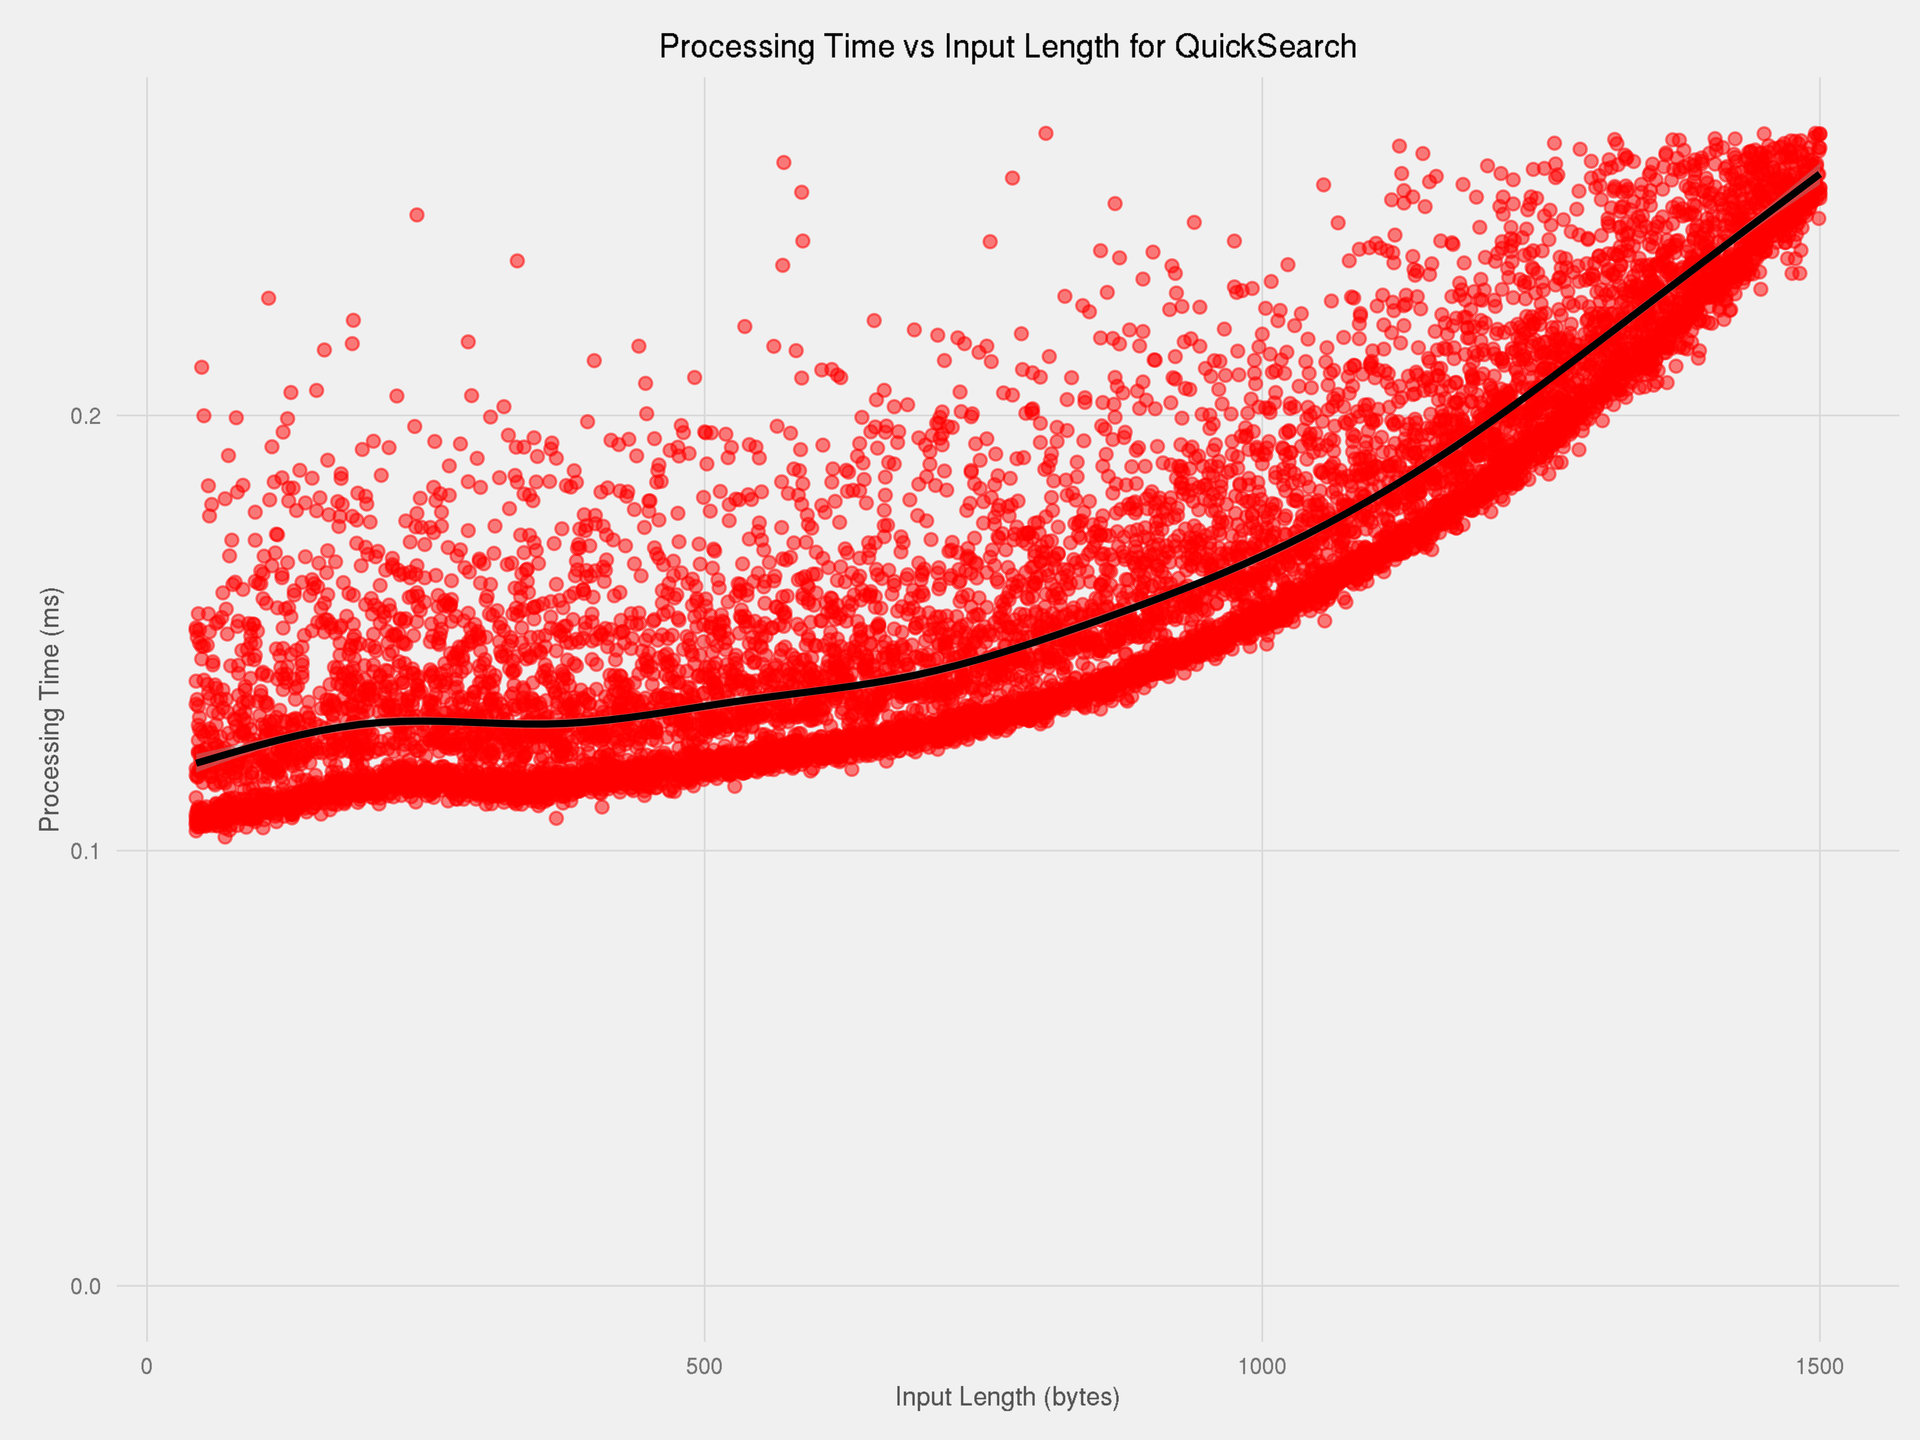
\includegraphics[width=\textwidth]{images/processing_speed_vs_input_length_no_matches_QuickSearch}
      \caption{QuickSearch}
      \label{figure-processingtimevslengthquicksearch}
  \end{subfigure}
  ~
  \begin{subfigure}[b]{0.48\textwidth}
      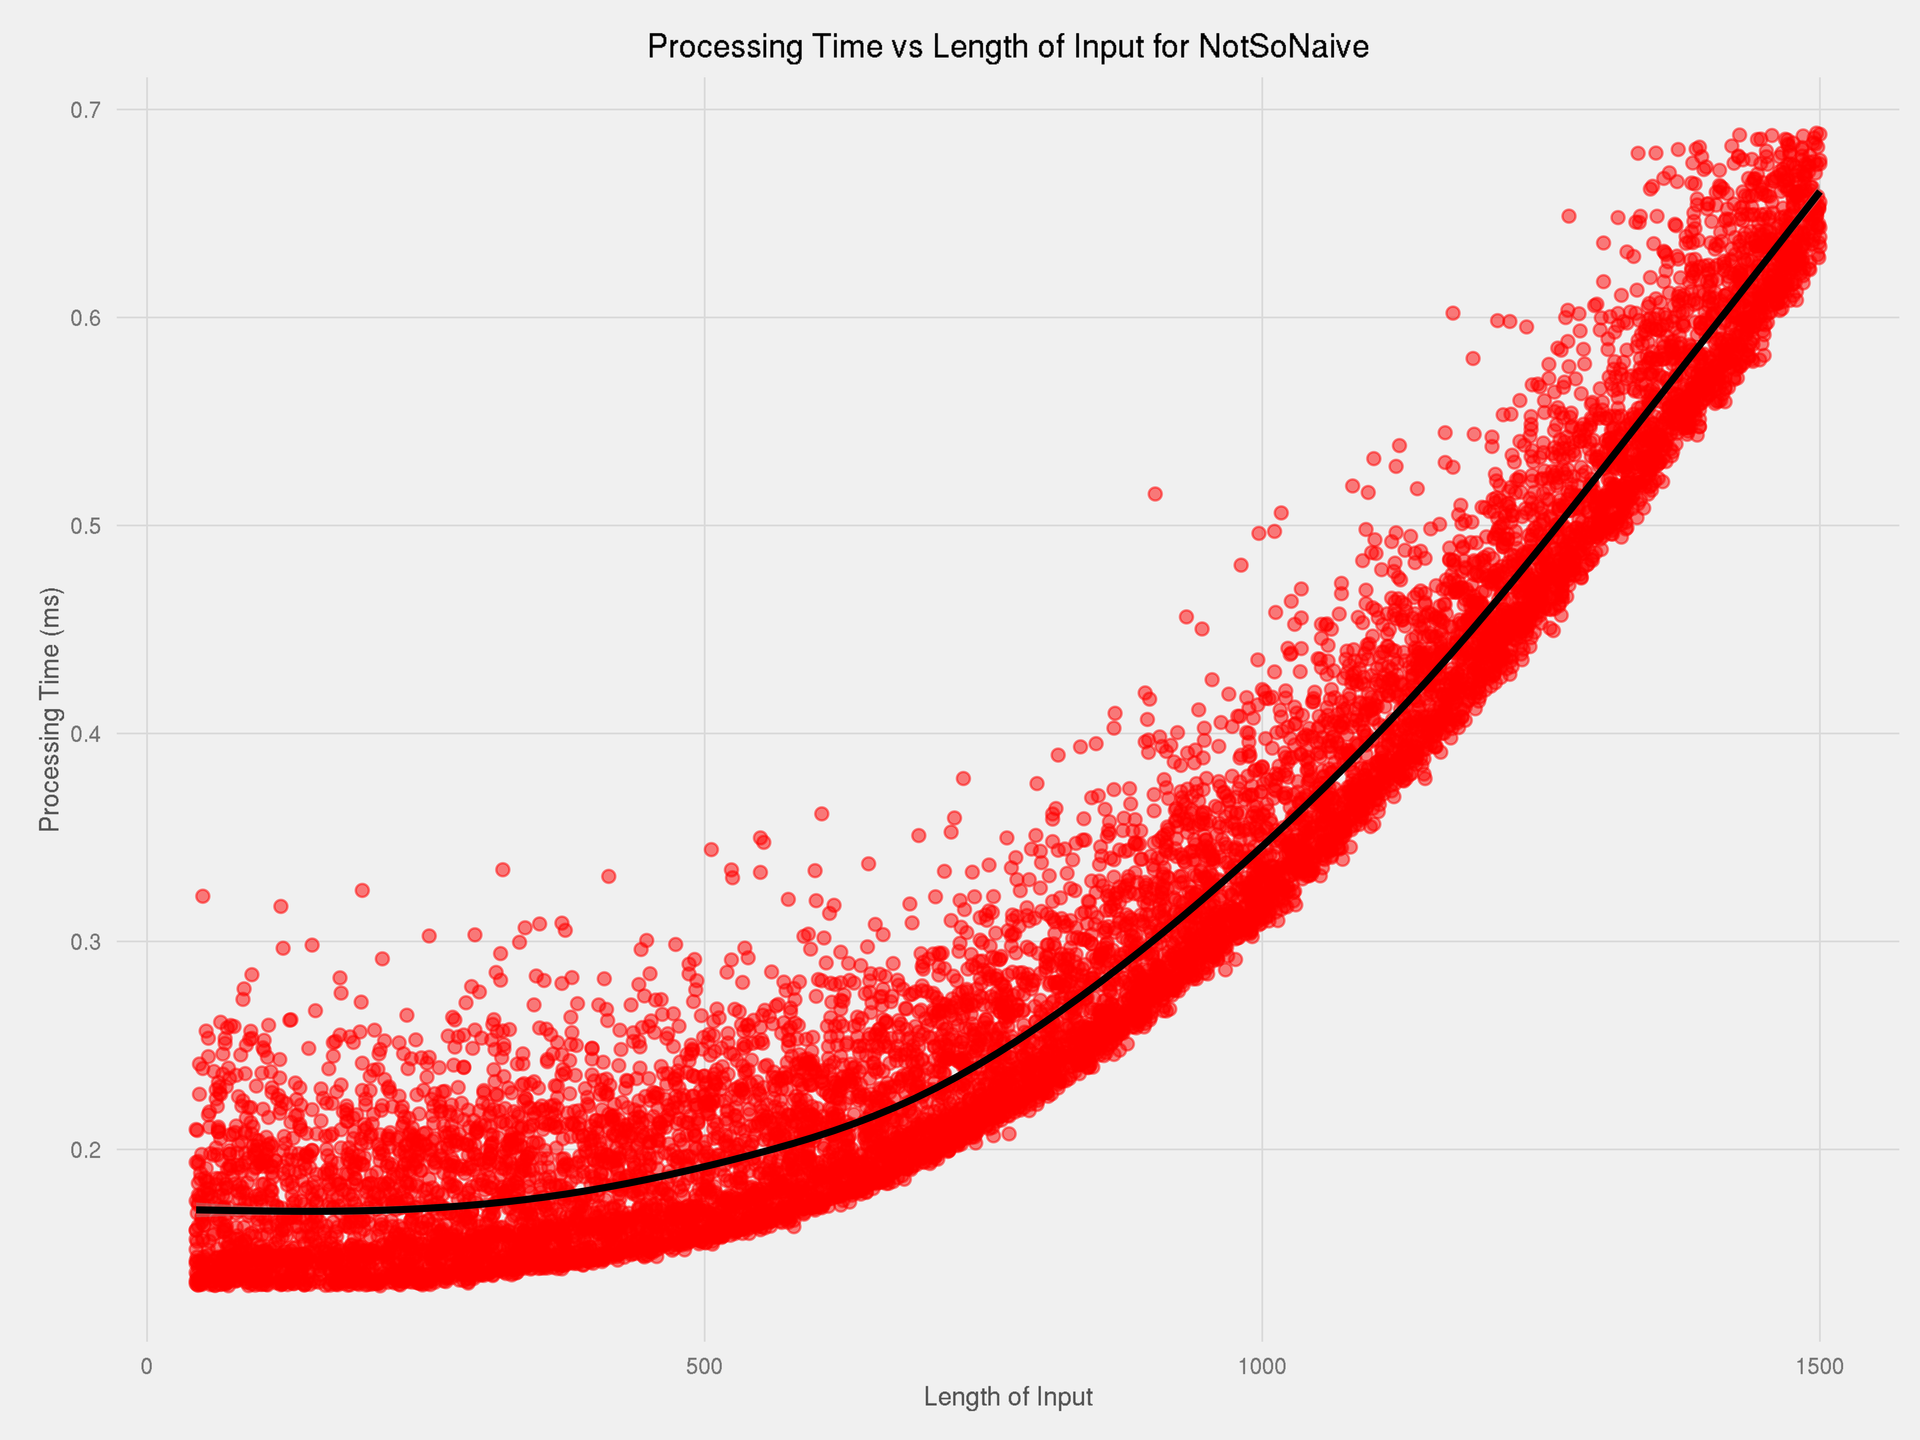
\includegraphics[width=\textwidth]{images/processing_speed_vs_input_length_no_matches_NotSoNaive}
      \caption{NotSoNaive}
      \label{figure-processingtimevslengthnotsonaive}
  \end{subfigure}
  \begin{subfigure}[b]{0.48\textwidth}
      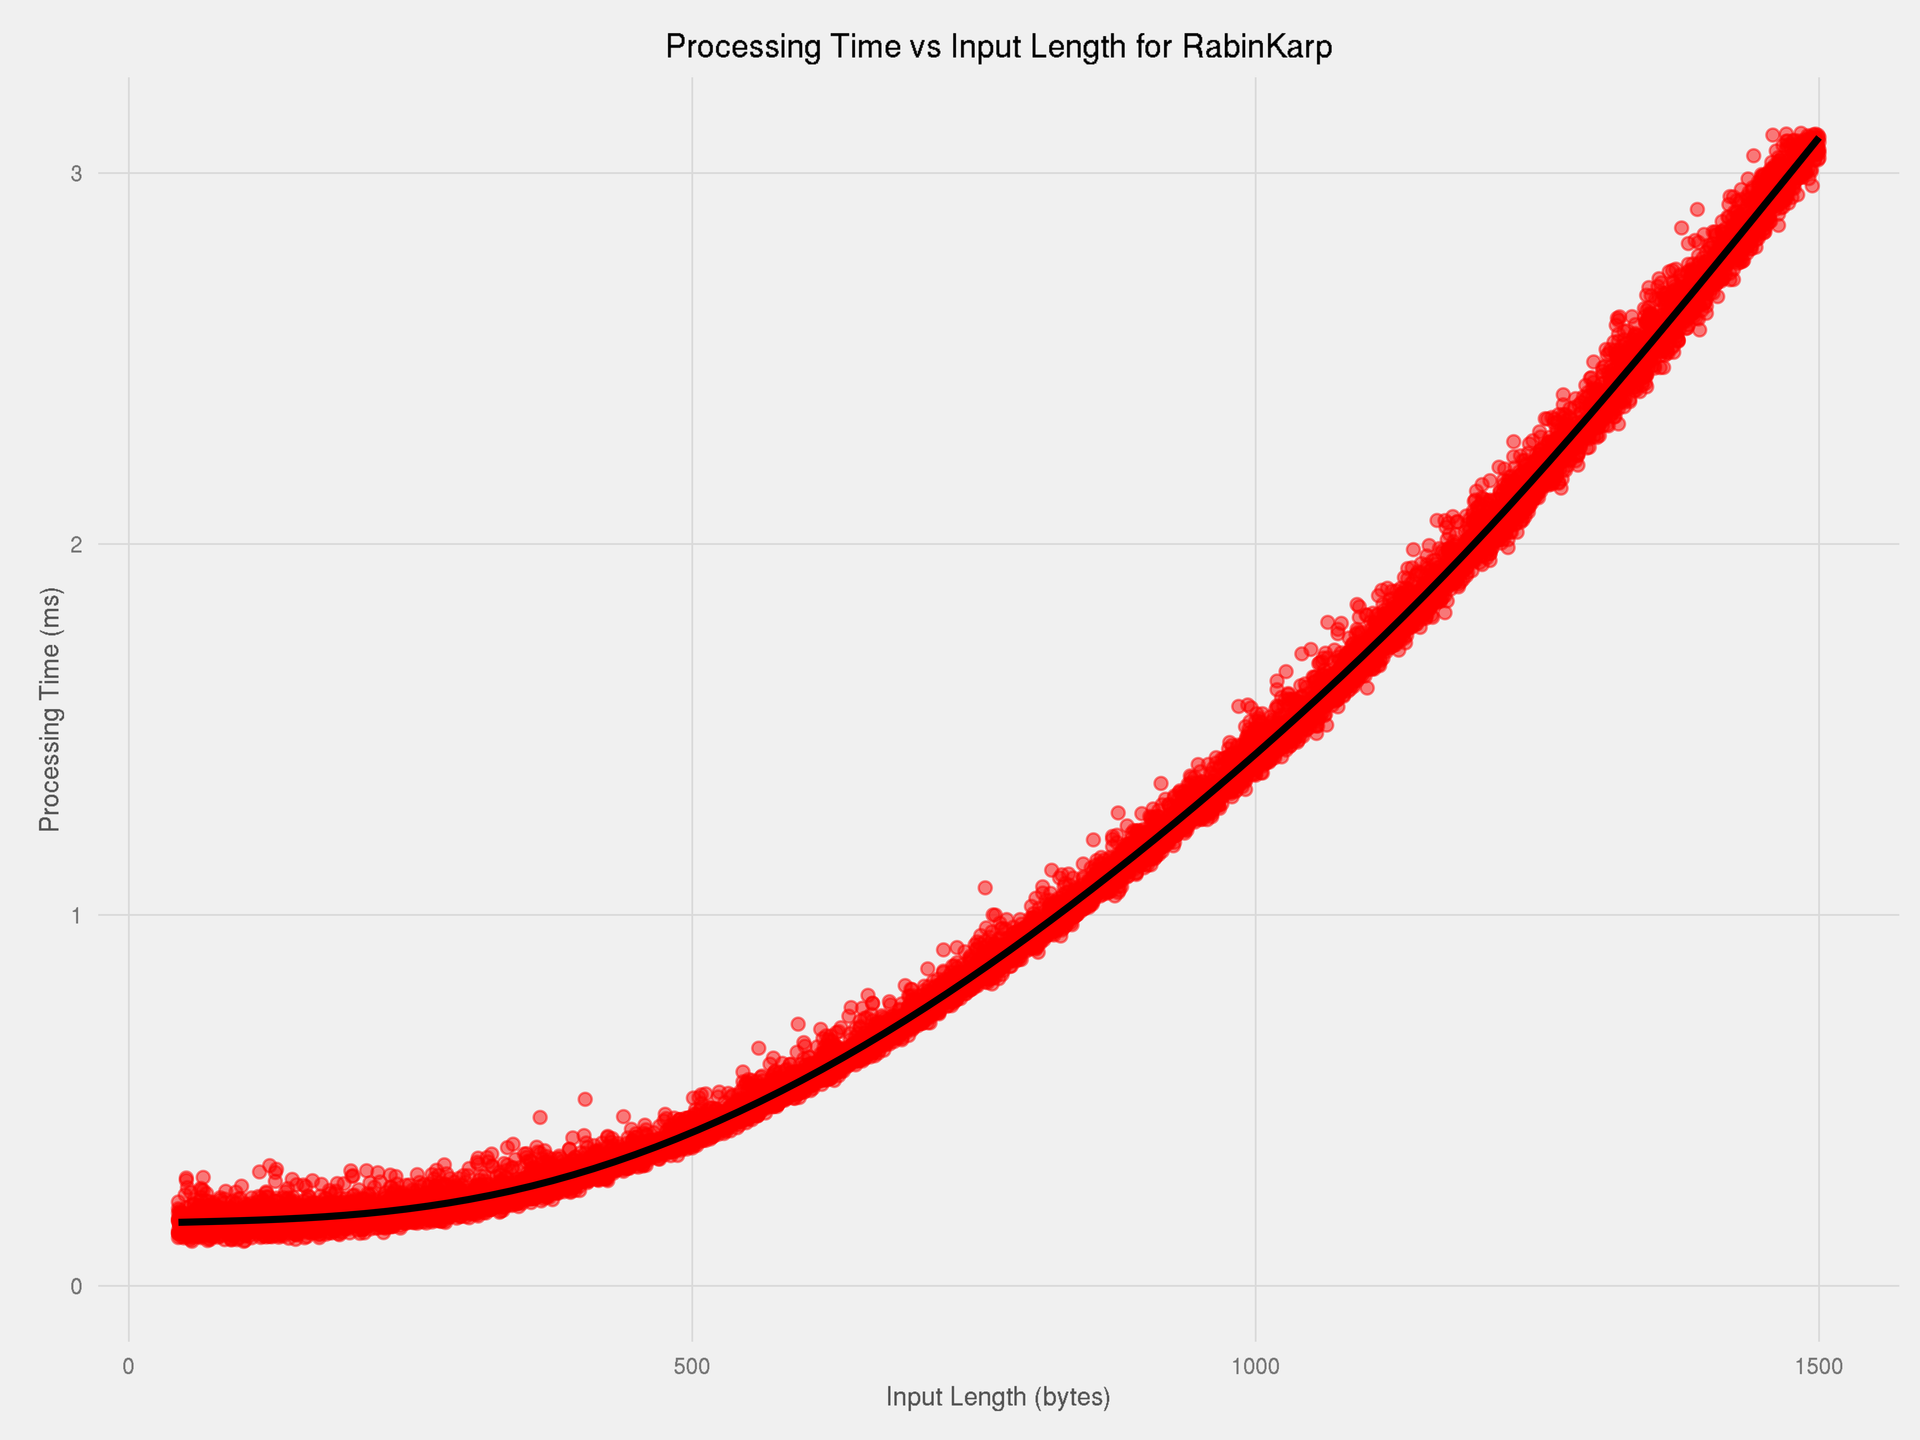
\includegraphics[width=\textwidth]{images/processing_speed_vs_input_length_no_matches_RabinKarp}
      \caption{RabinKarp}
      \label{figure-processingtimevslengthrabinkarp}
  \end{subfigure}
  \caption{Mean processing times versus input length for the Horspool, QuickSearch, NotSoNaive, and RabinKarp algorithms for \textit{Dataset C}.}
  \label{figure-individualalgorithmsvslength}
\end{figure}

From Figure \ref{figure-individualalgorithmsvslength}, it is clear that the processing times for Horspool and QuickSearch (Subfigures \ref{figure-processingtimevslengthhorspool} and \ref{figure-processingtimevslengthquicksearch} respectively) do not rise as quickly as those of NotSoNaive and RabinKarp (Subfigures \ref{figure-processingtimevslengthnotsonaive} and \ref{figure-processingtimevslengthrabinkarp} respectively) for inputs of greater length. Both NotSoNaive and RabinKarp show an exponential rise in processing times. 

Horspool and QuickSearch also show initial humps in processing speed around the 250 byte mark. This can be attributed to the overheard associated with each packet. For packets of more than 250 bytes, the processing speed relies more on the length of the packet then the initial - per-packet - overhead. This initial hump is not evident on either NotSoNaive nor RabinKarp; the reason for this is twofold. First, the speed of these algorithms is more affected by the input length, because of this an initial hump would be surpassed by the time it takes to process each packet. Second, the vertical scale of these two graphs is much larger than that Horspool or QuickSearch. Owing to that a small hump earlier on is less visible on a larger scale.


\section{Processing Speed vs Number of Matches}

For Section \ref{sec-processingspeecvsinputlength}, \textit{Dataset C} was created. It was designed in such a way that the number of matches in the input would not affect the processing speed. The processing speed was thus only affected by the length of the input and the algorithm used. In order to compare the processing speed against different numbers of matches, another Dataset needed to be created. \textit{Dataset D} contains 10000 DNS packets. Each 1500 bytes long. The payload in \textit{Dataset D} contains a mixture of randomized text and repeated strings of the rules. Each packet therefore contains between 0 and 1500 bytes of characters which are known to match with the rules used. This input data isolates the number of matches from the length of the input.

\begin{figure}[!htb]
  \centering
  \begin{subfigure}[b]{0.48\textwidth}
      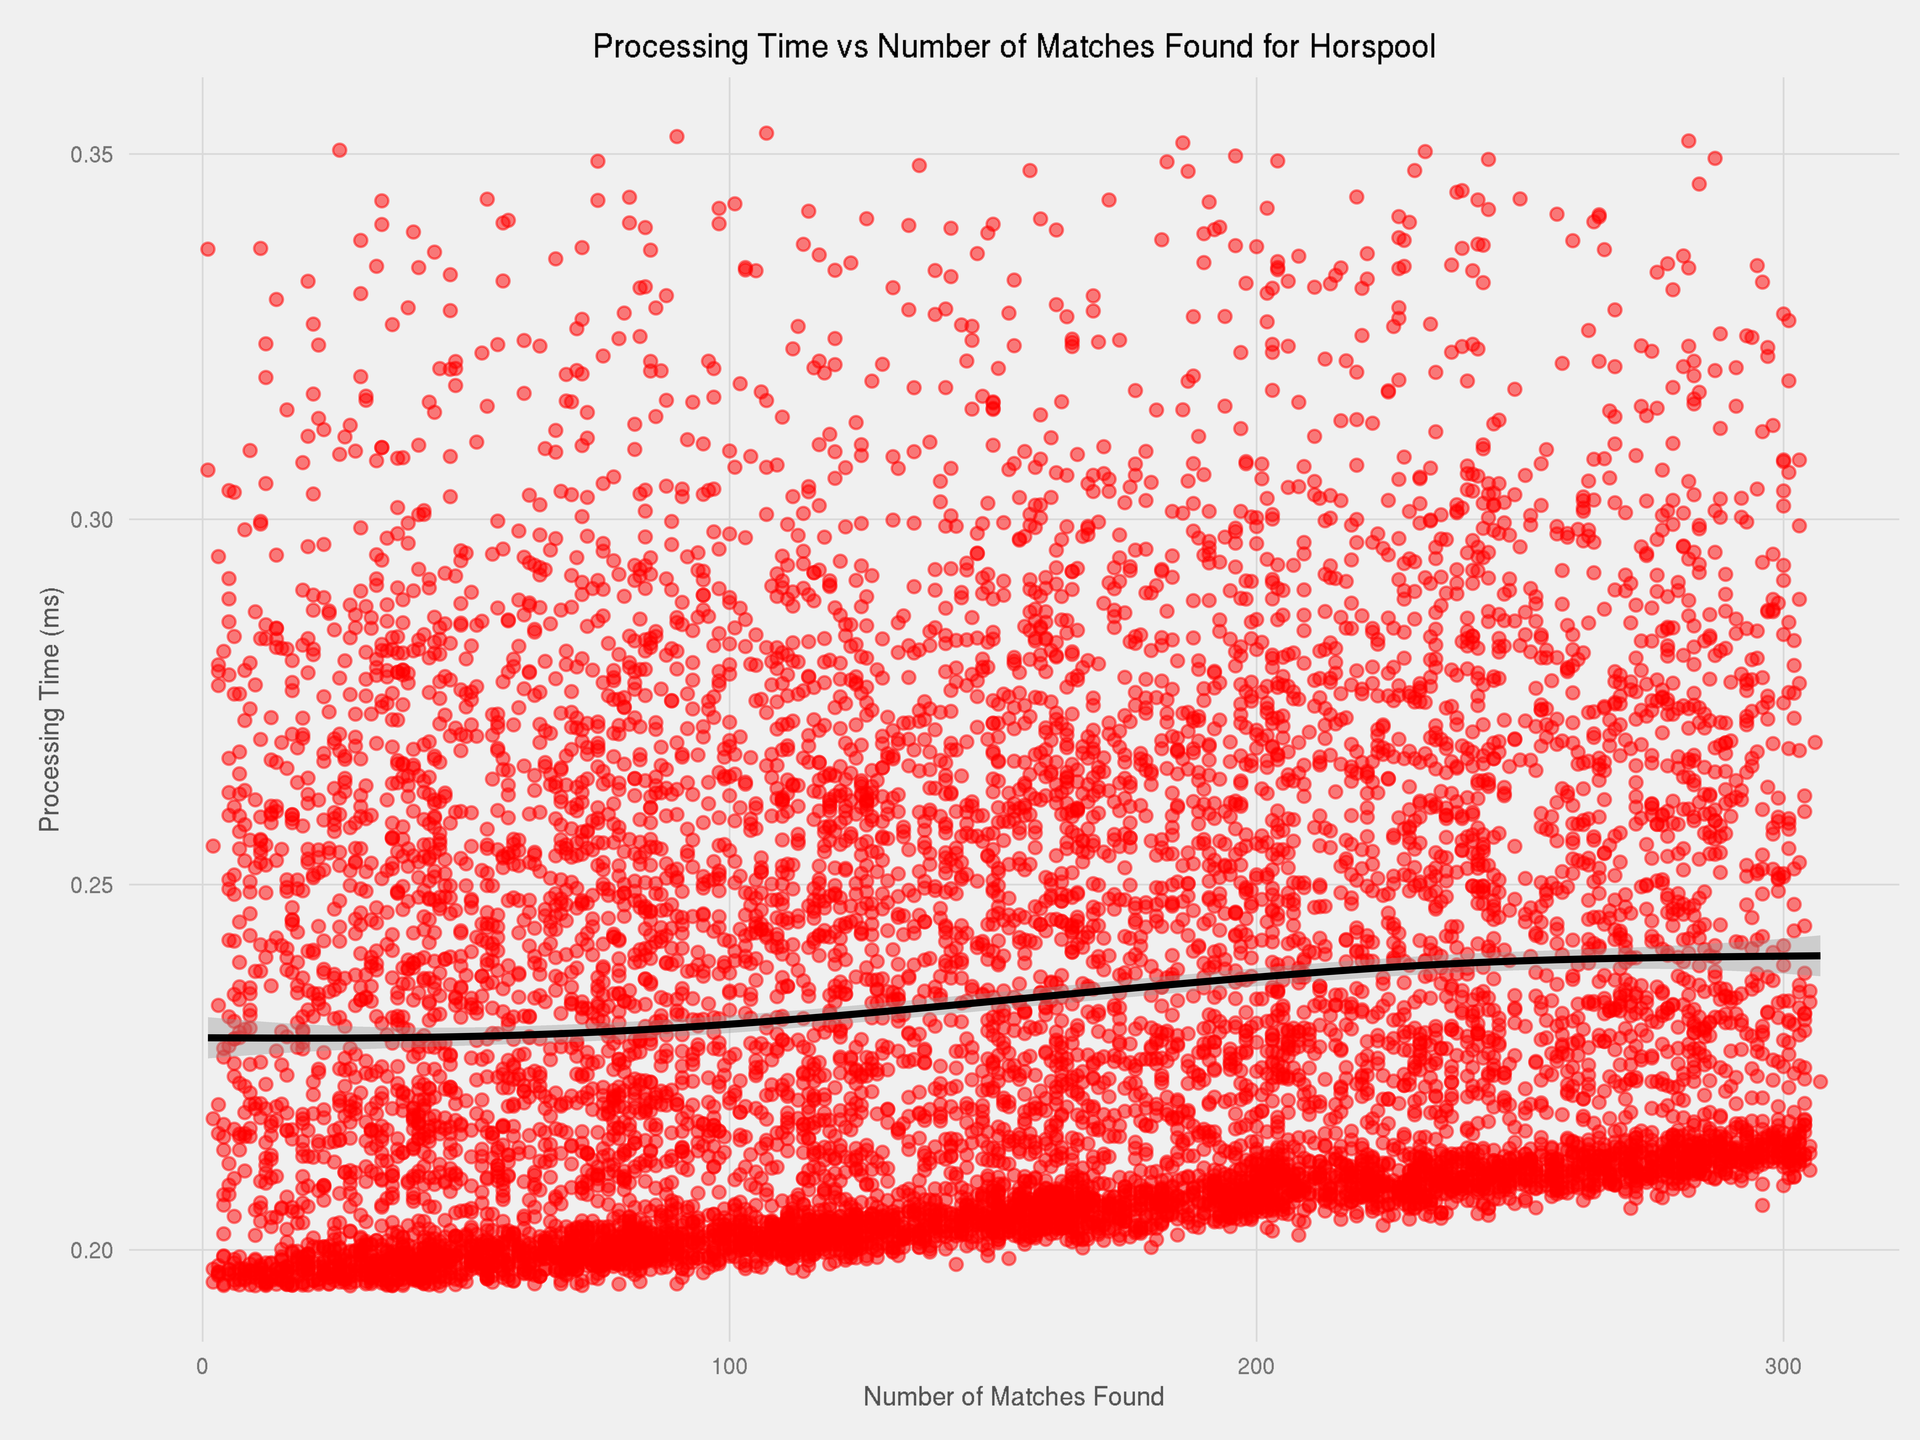
\includegraphics[width=\textwidth]{images/processing_speed_vs_num_matches_Horspool}
      \caption{Horspool}
  \end{subfigure}
  \begin{subfigure}[b]{0.48\textwidth}
      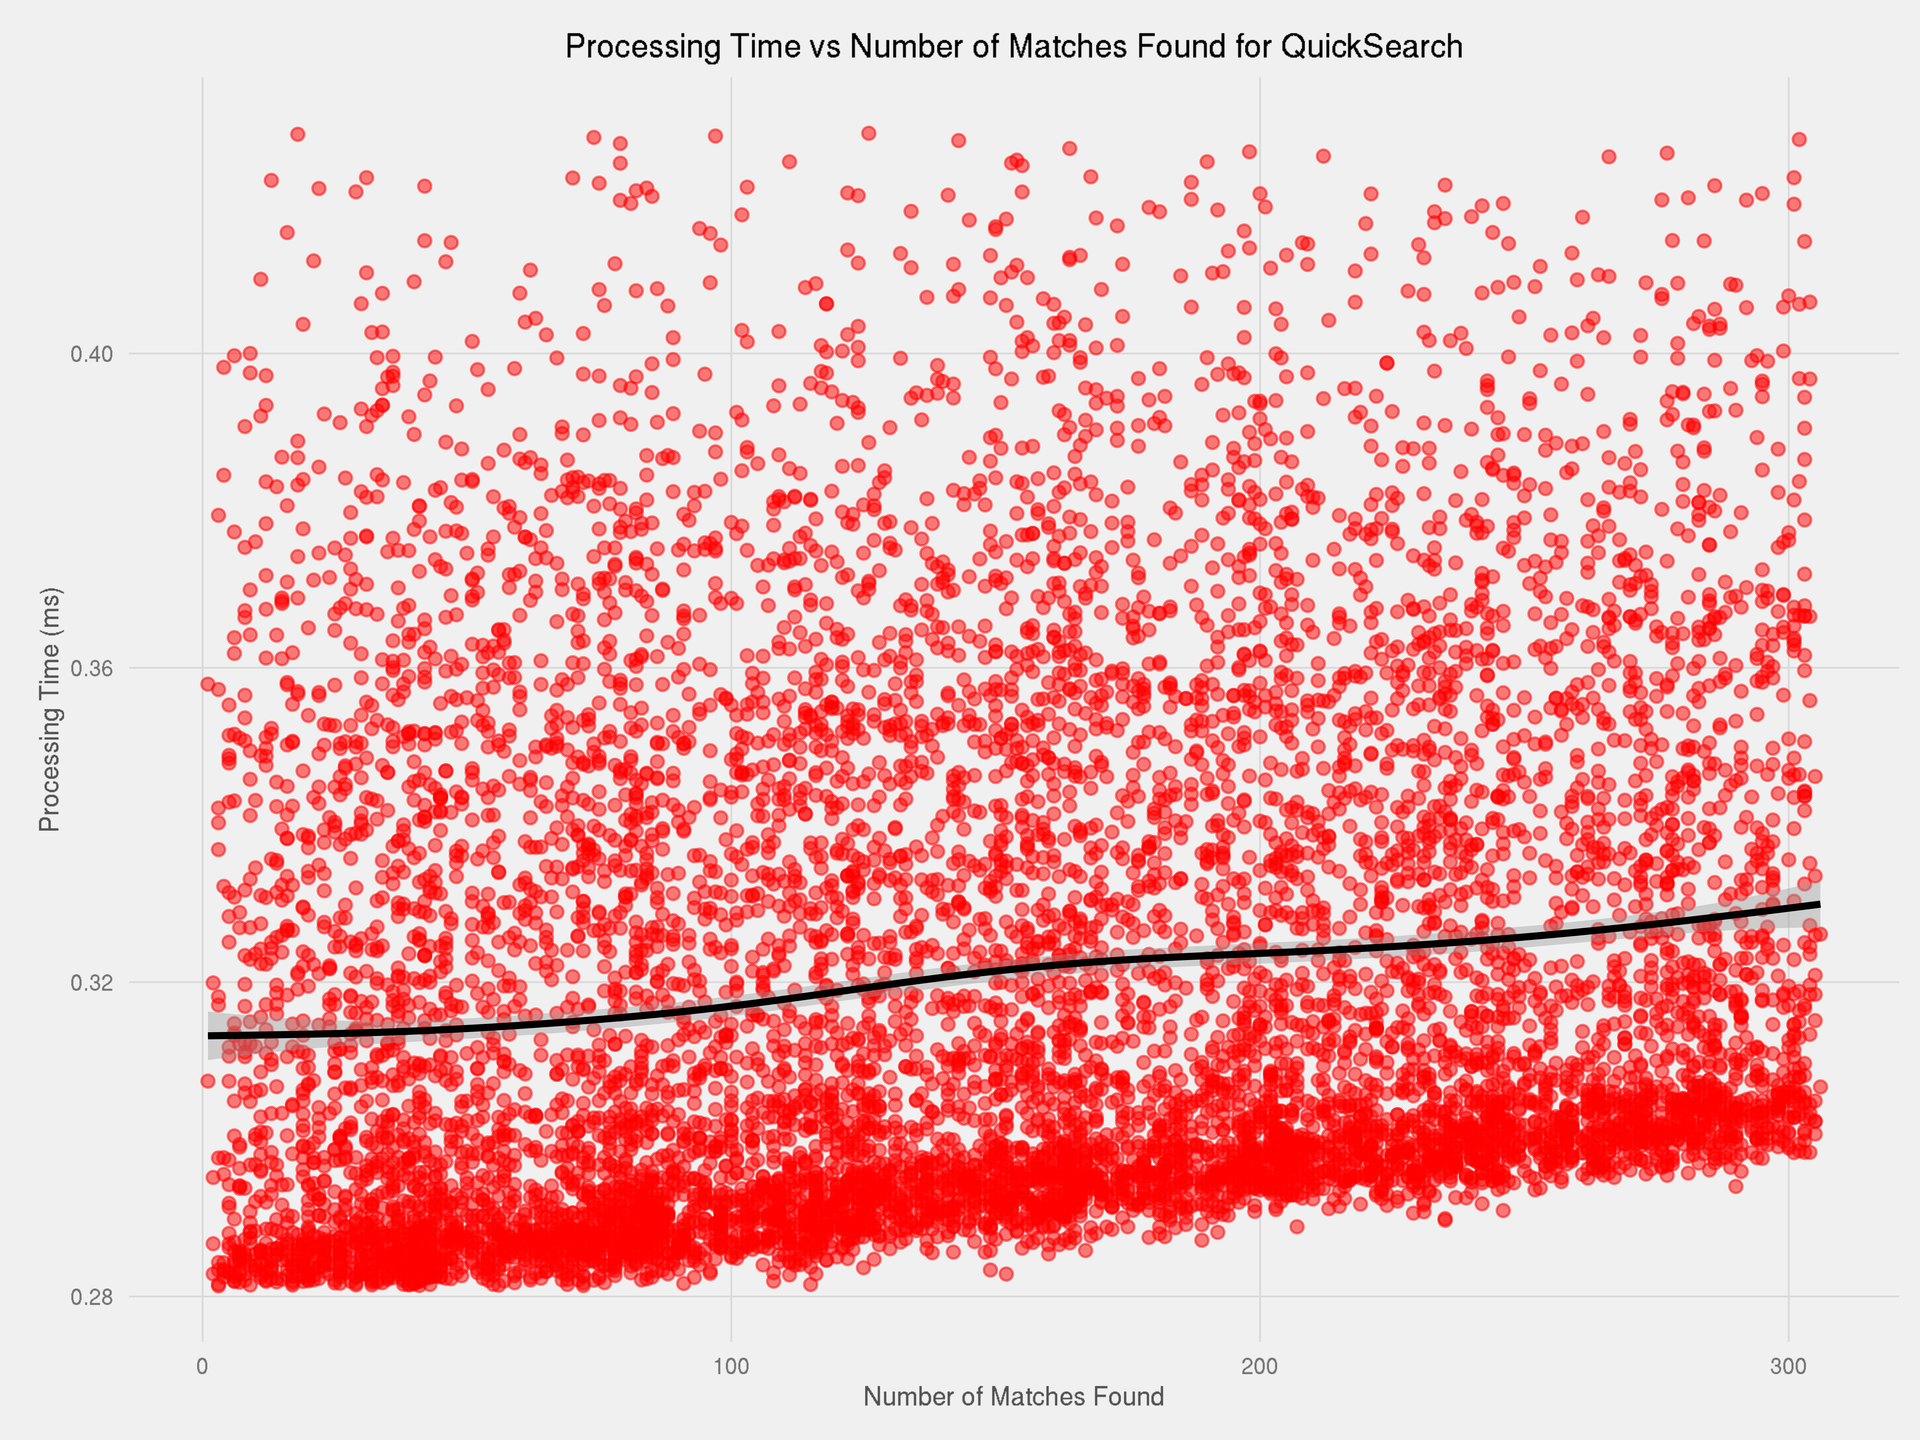
\includegraphics[width=\textwidth]{images/processing_speed_vs_num_matches_QuickSearch}
      \caption{QuickSearch}
  \end{subfigure}
  ~
  \begin{subfigure}[b]{0.48\textwidth}
      \includegraphics[width=\textwidth]{images/processing_speed_vs_num_matches_NotSoNaive}
      \caption{NotSoNaive}
  \end{subfigure}
  \begin{subfigure}[b]{0.48\textwidth}
      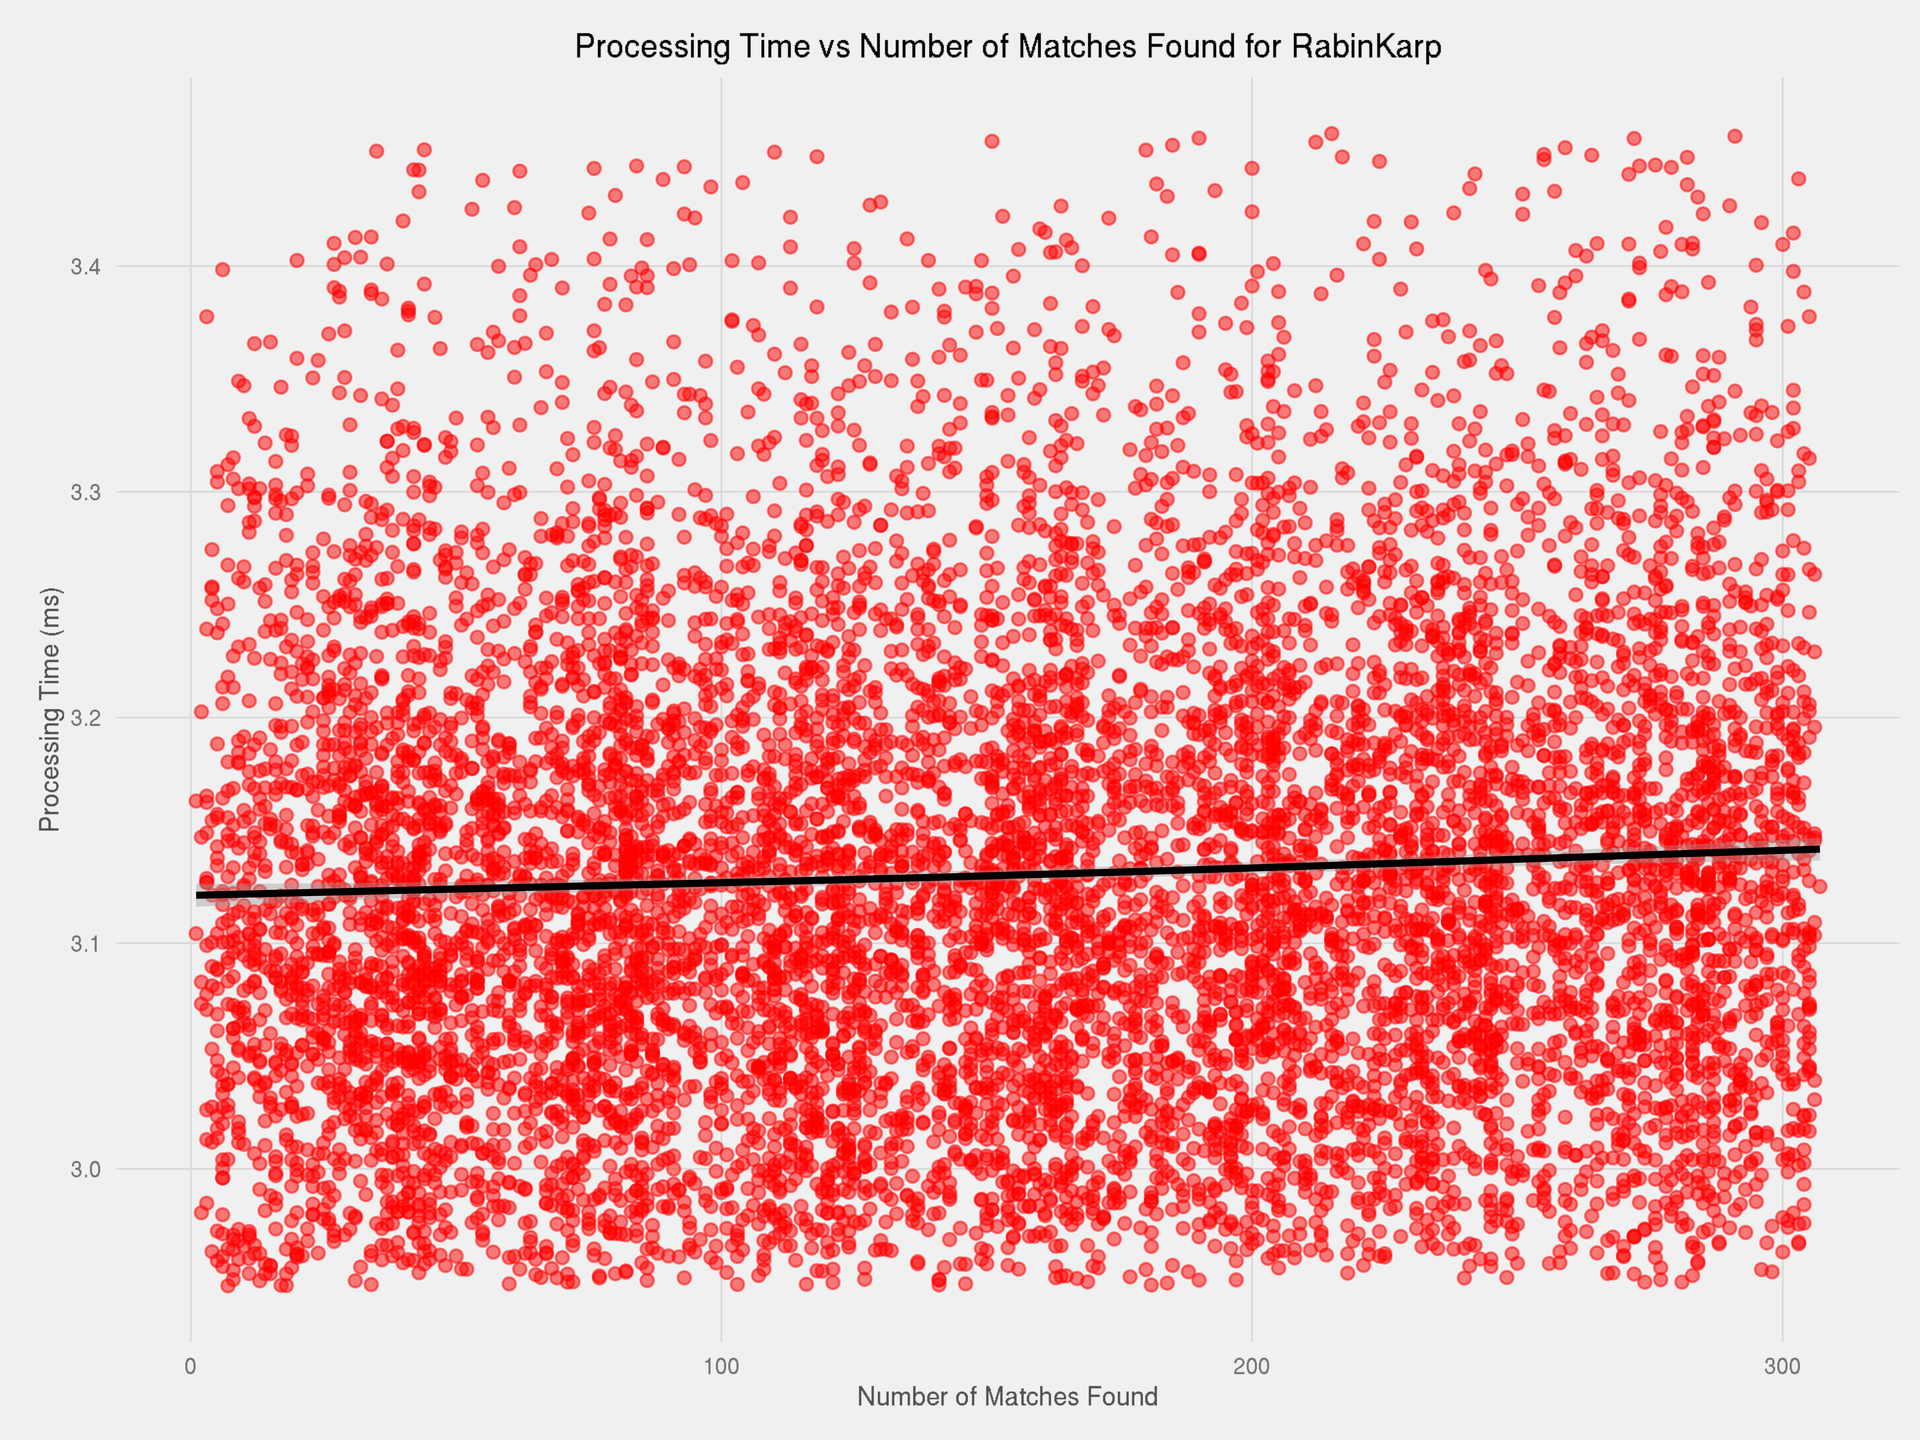
\includegraphics[width=\textwidth]{images/processing_speed_vs_num_matches_RabinKarp}
      \caption{RabinKarp}
  \end{subfigure}
  \caption{Mean processing times for each algorithm vs number of matches. \textit{Dataset D}.}
  \label{figure-individualalgorithmsvsnumberofmatches}
\end{figure}


\section{Parallelism}

In order to test how each of the algorithms performs under different levels of parallelism, a simple set of tests was devised. \textit{Dataset C} was selected as the input for the tests as it should not contain any matches.  The configuration file mentioned in \citet{hunt2016} allows the number of threads to be specified. The test computer has a total of 24 cores available and the test searches for each of the rules in parallel. In this test's case there were 40 rules. The following numbers of threads were selected to be tested: 1, 2, 4, 8, 16, 32, 64.

A overall speed increase should take place for thread numbers between one and sixteen. This is still below the twenty four cores available and so each thread can occupy a separate core. At thirty two threads there are now more threads than available cores and so threads have to share processing time on cores. This could lead to further overhead as the processor switches contexts depending on which thread has been scheduled.

\begin{figure}[!htb]
  \centering
  \begin{subfigure}[b]{0.48\textwidth}
      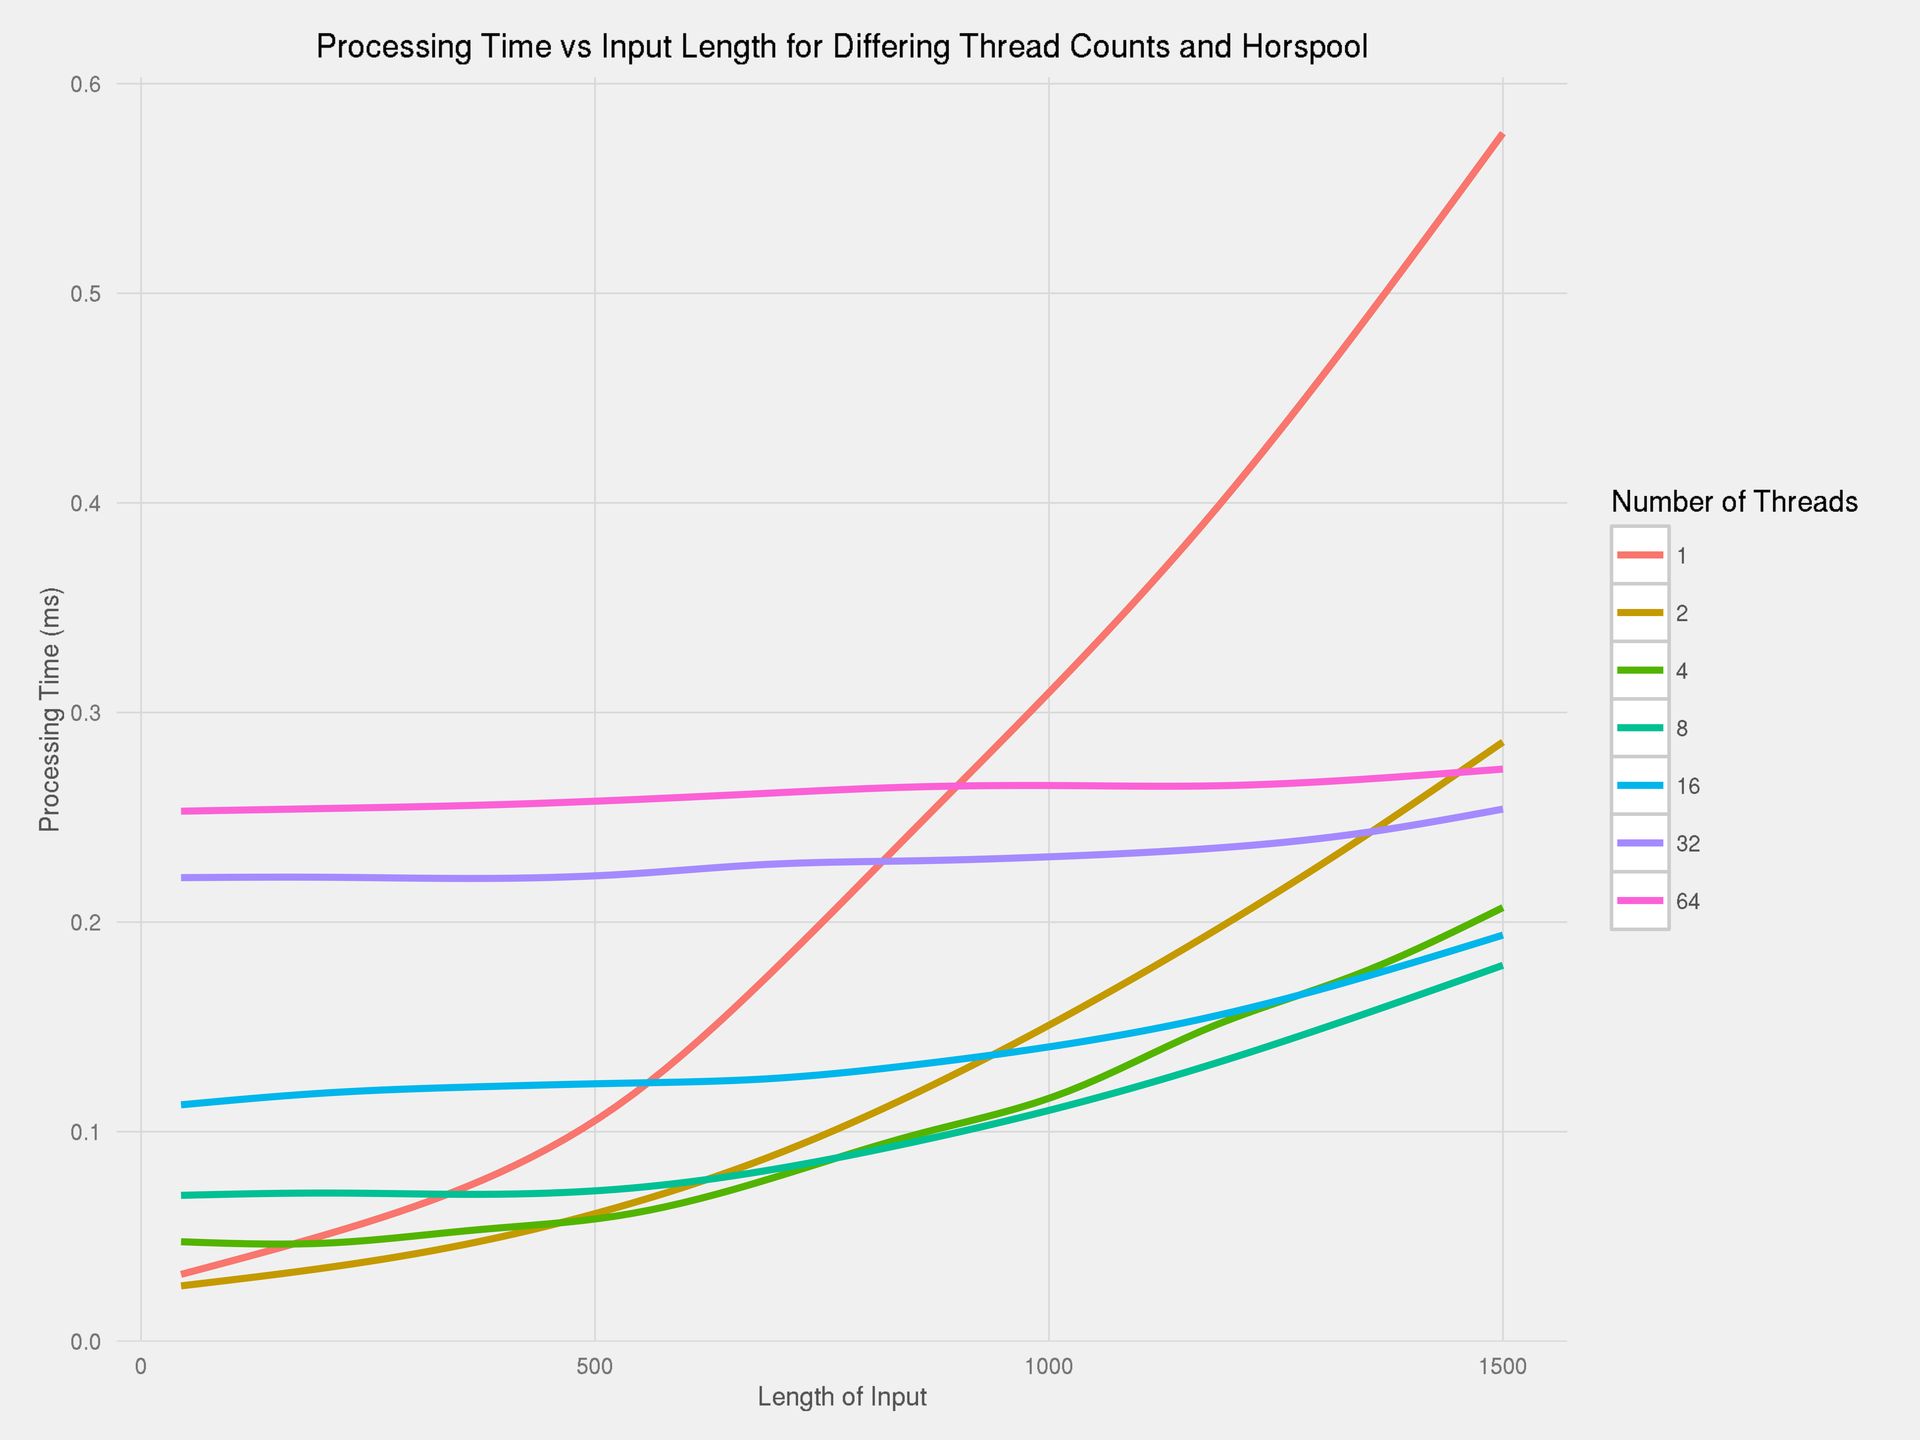
\includegraphics[width=\textwidth]{images/scatter_elapsed_vs_input_length_many_cores_Horspool}
      \caption{Horspool}
  \end{subfigure}
  \begin{subfigure}[b]{0.48\textwidth}
      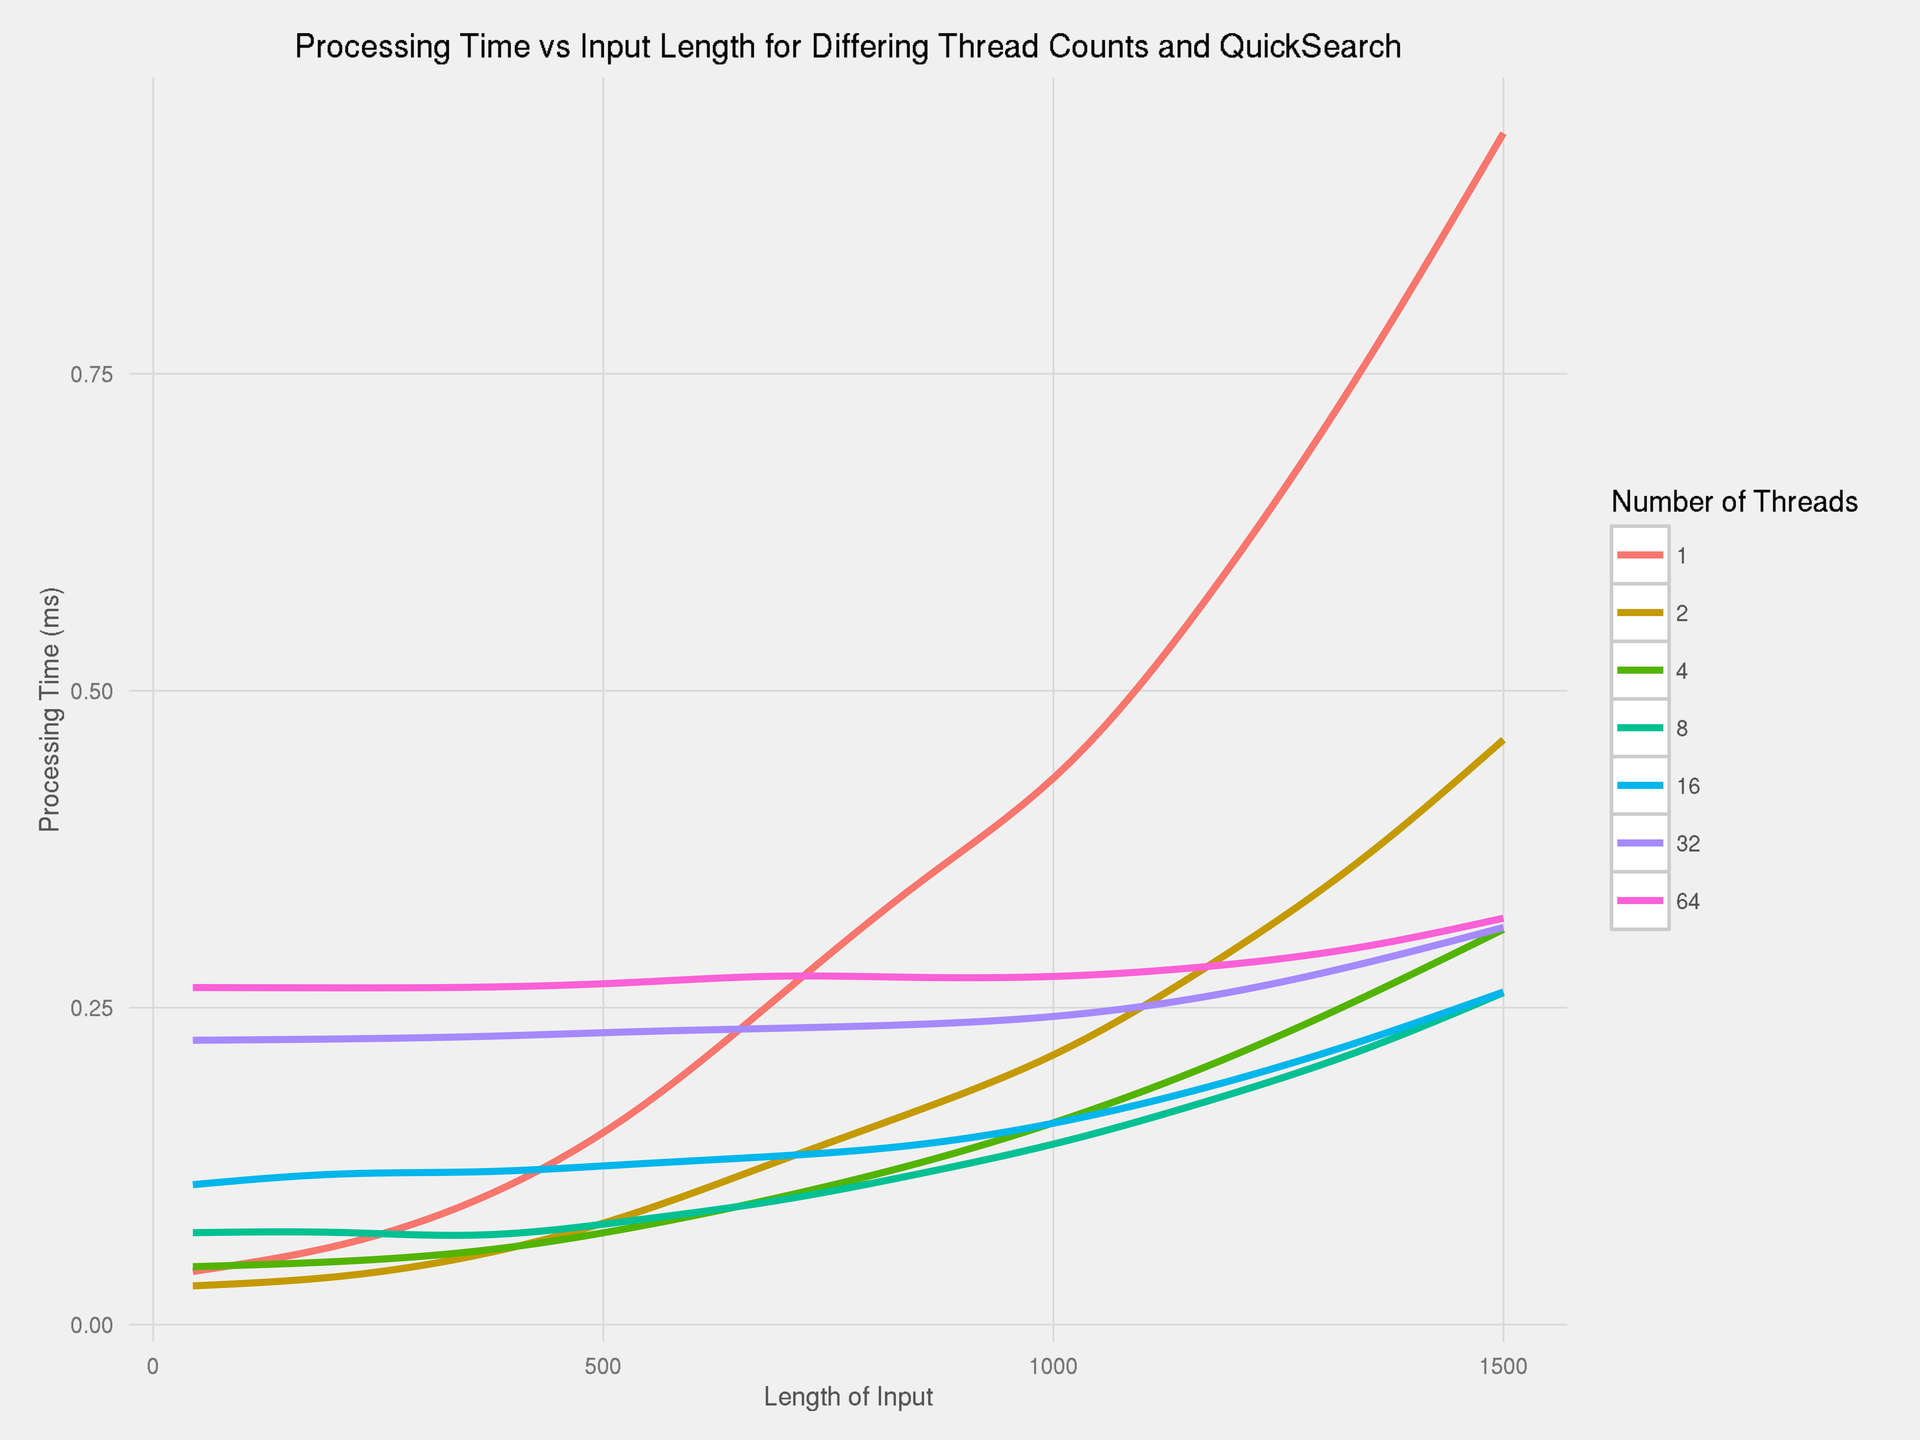
\includegraphics[width=\textwidth]{images/scatter_elapsed_vs_input_length_many_cores_QuickSearch}
      \caption{QuickSearch}
  \end{subfigure}
  ~
  \begin{subfigure}[b]{0.48\textwidth}
      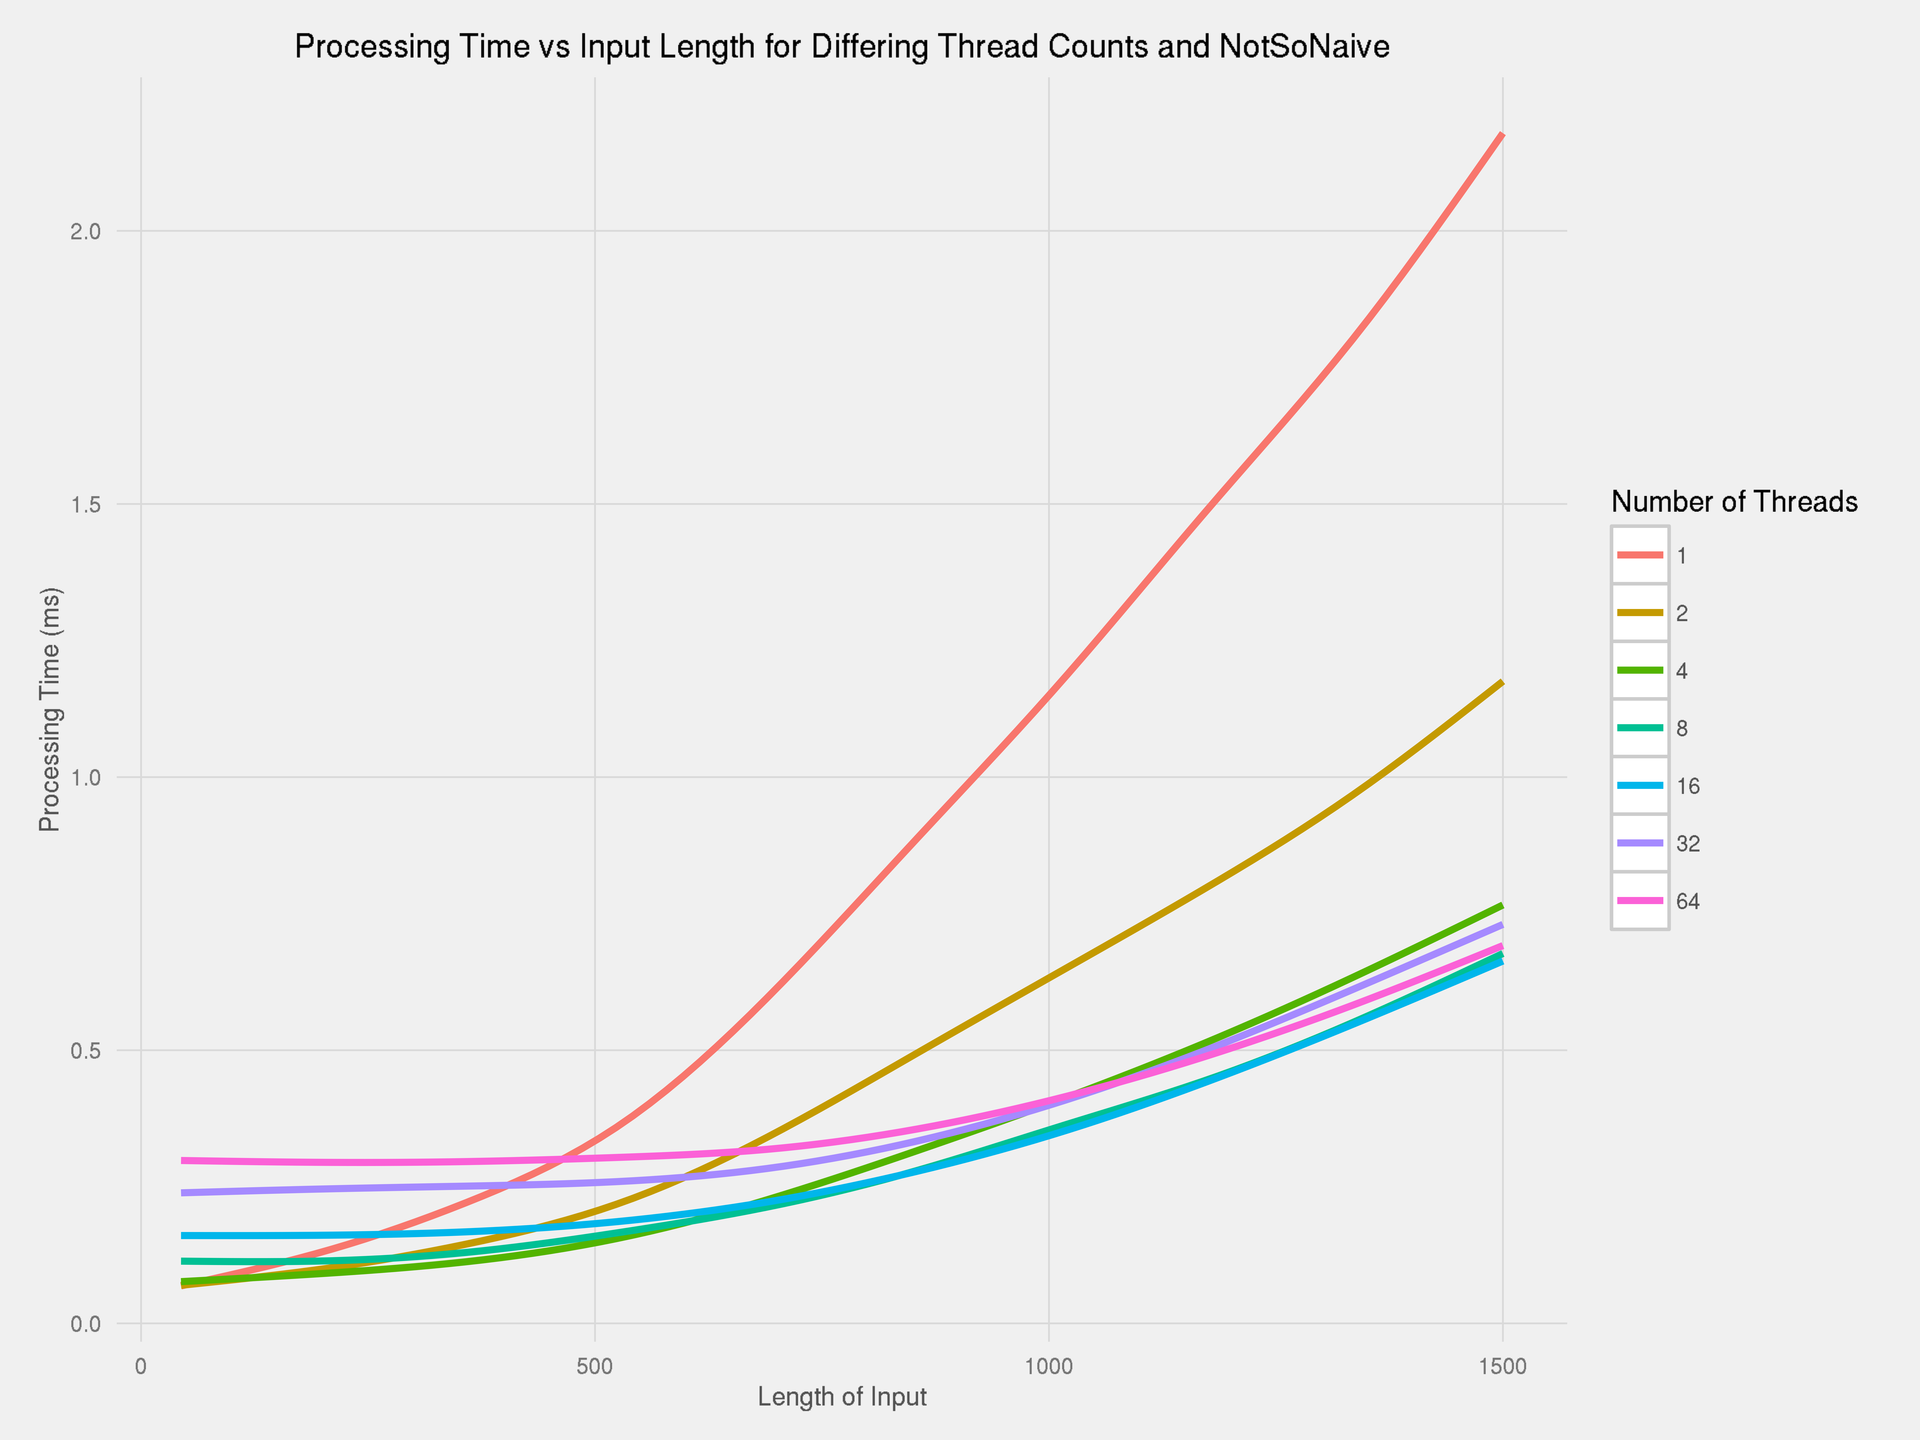
\includegraphics[width=\textwidth]{images/scatter_elapsed_vs_input_length_many_cores_NotSoNaive}
      \caption{NotSoNaive}
  \end{subfigure}
  \begin{subfigure}[b]{0.48\textwidth}
      \includegraphics[width=\textwidth]{images/scatter_elapsed_vs_input_length_many_cores_Rabinkarp}
      \caption{RabinKarp}
  \end{subfigure}
  \caption{Mean processing times for each algorithm vs number of matches. \textit{Dataset D}.}
  \label{figure-processingtimevsinputlengthdifferentcores}
\end{figure}

Figure \ref{figure-processingtimevsinputlengthdifferentcores} provides some very interesting results. As expected, single core implementations are the slowest overall and speed increases are realised as the length of the packets grow. This result is unsurprising as longer packets mean that the overhead of switching threads is reduced over time. Also as expected, the lower thread counts are more efficient for smaller packets but they lose efficiency as the length increases. On our particular test computer, between eight and sixteen threads proves to be the most efficient for longer packet lengths. At about 770 bytes either four or eight threads is most efficient for the majority of algorithms.



\bibliographystyle{plainnat}
\bibliography{references}

\end{document}